
	\chapter{Cadre du projet }
	\newpage
	
	
	\section{Introduction }

	
	\section{Problématique }
	Depuis des temps immémoriaux, l'agriculture était très importante dans la mesure où elle faisait partie intégrante de la vie humaine et demeure d’une grande importance économique et sociopolitique du fait de sa contribution à la réalisation des objectifs nationaux en matière de sécurité alimentaire, de création de revenus, d’emplois, d’équilibre régional et de gestion des ressources naturelles. Néanmoins ce secteur central a étalé une faiblesse importante mondiale et régionale de compétitivité sur les marchés nationaux et internationaux suite à un manque de la technique et de l'innovation qui reflète une faible production et l'absence de qualité des produits agricoles d'organisations professionnelles bien développée . Les agriculteurs doivent constamment faire des miracles pour trouver des solutions à de nouveaux problèmes. Les défis à relever à l'avenir peuvent être très différents des problèmes rencontrés aujourd’hui. Pour cette raison-là, L'agriculture a connu de nombreuses crises vue qu’ils utilisent les mêmes moyens sans innover de nouvelles technologies ni augmenter sa productivité.
	
	Ces dernières années, le monde a été confronté à une baisse importante de la production agricole. Par exemple, Au Brésil, le premier producteur d’oranges dans le monde avec plus de 19 millions de tonnes d'où proviennent plus de la moitié des fruits utilisés pour fabriquer les jus consommés à travers le monde, la situation est particulièrement critique. La production d'oranges risque d'être la plus faible depuis plus de vingt ans, d'après les estimations du département américain de l'Agriculture (Usda)[5]. En Tunisie, la production d'agrumes de la campagne 2017/2018 a fortement chuté à 38,2 \%, soit 346 000 tonnes. Cette baisse de production est due à une baisse du maltais (49\%), de la clémentine (38\%) et du nombril (31\%)[5].
	
	En plus, récemment avec le covid19 le secteur agricole face à d’autres problèmes et d’autres challenges a cause de cette crise sanitaire. Il a perturbé le fonctionnement de l'agriculture et du système alimentaire en perturbant le processus de production menant au centre de consommation. En raison des restrictions, il y a plus de travailleurs ni des ouvrières dans de nombreux secteurs et domaines, ce qui peut facilement affecter la production et les économies mondiales et régionales. Le confinement des pays et la fermeture des frontières ont une forte incidence sur la rapidité et la flexibilité d’un secteur initiale, l’agriculture, vue que y'a un manque de main d'œuvres et l'absence d'innovations alternatives ce qui peut refléter un ralentissement de la production agricole.
	
	\section{Solution proposée }
	Après avoir étudié attentivement ce sujet et l'observation et l'analyse des problèmes qui résultent de ce sujet. Nous avons bien conclu qu'il faut créé une progression au niveau de ce secteur et crée des solutions qui peuvent augmenter la qualité et la production de l'agriculture et aider les agriculteurs à avoir une progression au niveau de la compétitivité dans ce domaine-là. Aujourd'hui, l'agriculture est un secteur énorme, et donc un autre domaine est nécessaire pour développer les avantages de l'agriculture et obtenir des résultats plus précis, de sorte que l'importance de la technologie doit être prise en compte et ça va permettre d’évoluer l’agriculture afin d’améliorer le quotidien de chaque producteur ainsi que leur rendement. 
	
	Ce dernier a besoin d'aide pour connaître ses estimations de production, ce qui n’est pas facile avec la main-d'œuvre. Cela peut aussi prendre du temps, mais avec la technologie, on peut changer la situation, gagner un temps considérable et optimiser le rendement de ses parcelles grâce à ces appareils qui permettent une vue aérienne précise et la collecte de nombreuses données  sans le perdre et offrir aux agriculteurs un regard plus holistique sur leurs fermes et la capacité de vérifier la santé de leur bétail. Les progrès de la technologie agricole peuvent ainsi aider les agriculteurs à mesurer, suivre et améliorer continuellement leur empreinte environnementale et soutenir la rentabilité des exploitations en maintenant une agriculture viable pour les générations futures.
	
	Dans ce contexte, nous avons vu que La combinaison de produits à valeur agricole et d’innovation technologique ouvre la voie à un avenir plus vert, plus productif et durable c’est pour cela nous avons mis en place un système innovant focalisé sur l'application d'un drone pour la détection des oranges. Ce drone peut filmer pour réaliser une inspection visuelle des arbres et accéder à des zones compliquées d’accès. Effectivement, cette technique présente plusieurs avantages pour le monde agricole y compris la croissance de la production agricole en évaluant les prévisions de rendement, le suivi ou bien évaluation des cultures, la réduction des risques liés aux cultures, la prévision des catastrophes et l’optimisation des coûts. 
	Ce système est divisé en deux volets :
	\begin{itemize}
		\item  drone 	
		\item détection des oranges
	\end{itemize}
	
	
	\section{Objectif }
	L'objectif de notre projet de fin d’étude est d’utiliser les nouvelles technologies pour améliorer les performances économiques et environnementales des productions agricoles. Afin de s’organiser de manière appropriée, les agriculteurs ont besoin d’anticiper leur production. Mais le comptage des fruits est une tâche qui prend beaucoup du temps. Notre projet sous le nom « AGRI Drone » - est consacré à optimiser ce temps perdu par le développement d’un système automatisé intégré dans un drone pour le comptage des oranges sur l’arbre. 
	
	
	Ce système va mettre au point une méthode de travail plus efficace et bien précis qui utilise l’intelligence artificielle pour permettre aux fournisseurs de produits agricoles à optimiser leurs récoltes et à planifier leurs ventes sur le marché. La technologie des drones pourrait aider les agriculteurs du monde entier à surveiller la croissance de leurs cultures, lutter contre les nuisibles, et bien plus encore. Grâce à la caméra et aux capteurs embarqués, le drone peut mesurer de nombreux indicateurs de l'état et des besoins de la plante . En fait, notre systéme fournit des informations plus précise et une variété de donneés.
	
	Bien que le prélèvement ait été exécuté manuellement, les informations recueillies par le drone permet aux agriculteurs d'identifier les zones à surveiller ou à traiter, de déterminer l'intervention la plus appropriée et de réduire la quantité de traitement utilisée. Tout cela sera facile et nous fera gagner de temps non négligeable avec cette nouvelle innovation.
	
	
	
	\section{Méthodologie de gestion de projet }
	\subsection{Choix de méthodologie }
	Afin d'assurer le bon déroulement des différentes étapes dans notre projet, nous avons choisi la méthode Agile Scrum pour gérer notre travail, concevoir et développer notre système pour des raisons claires est vraiment le processus Scrum s'inscrit parfaitement dans la décomposition de notre projet de fin d'études, qui s'appuie sur des avantages suivants :
	\begin{itemize}
		\item Plus de flexibilité et de réactivité.
		\item Traduire et organiser le projet de façon simple, transparente et pragmatique.
	\end{itemize}
	
	\subsection{C'est quoi Scrum }
	Scrum est la méthode agile la plus utilisée. A l'instar des autres méthodes agiles, Scrum est une démarche de gestion de projet qui fait du client (ou utilisateur) le principal pilote de l'équipe en charge des développements. [6]
	\subsection{Présentation de la méthodologie scrum }
	La méthode SCRUM implique que le projet progresse à travers la mise en place de séries de « sprints ». À chaque lancement d’un sprint, une réunion de planification est organisée afin que chaque membre de l’équipe puisse s’engager sur le nombre de tâches qu’il pourra exécuter, ainsi que sur la création du « sprint blacklog ».
	Chaque jour du sprint, tous les membres de l’équipe (ainsi que le responsable produit et le SCRUM Master) doivent assister à la réunion SCRUM quotidienne. Cette dernière ne doit pas durer plus de 15 minutes, et permet aux membres de l’équipe de partager avec les autres ce qu’ils ont fait la veille, ce sur quoi ils travaillent le jour même, ainsi que l’identification de tout problème pouvant entraver le bon déroulement du sprint. Cette réunion permet ainsi de synchroniser tous les membres de l’équipe.
	
	
	La fin d’un sprint est marquée par une session de débriefing permettant de présenter le travail achevé au responsable produit, et de partager des informations pouvant influer sur le sprint suivant.[7]
		\begin{figure} [h]
		\begin{center}
			\centering
			\includegraphics[width=1.1\linewidth]{Images/Méthode Scrum}
		\end{center}
		\caption{Méthode scrum}
	\end{figure}
	
	\subsubsection{Product owner }
	Personne ayant la responsabilité de produire et de maintenir à jour le carnet de produit. C'est lui qui détermine les priorités et qui prend les décisions d'orientation du projet .
	\subsubsection{Scrum master  }
	Membre de l'équipe dont l'objectif principal est de la protéger des perturbations extérieures. Il est complètement transparent pour la communication entre l'équipe et les clients et n'a aucun pouvoir hiérarchique sur l'équipe. C'est en revanche un facilitateur pour les problèmes non techniques de l'équipe .
	\subsubsection{Product backlog  }
	Liste des fonctionnalités, des fonctions, des exigences, des améliorations et des correctifs qui sont nécessaires à l'évolution du produit , celui-ci est dynamique sur tout le cycle de vie du produit.
	\subsubsection{	Sprint backlog }
	Liste des tâches à accomplir pendant un sprint. Elles correspondent à la réalisation des éléments de carnet de produit affectés au sprint .
	\subsubsection{Sprint }
	Nom d'une itération dans Scrum. Cette itération dure 1 mois maximum en théorie, mais en pratique entre 2 et 4 semaines. Pendant une itération, l'équipe doit développer la liste d'éléments du carnet de produit qui a été définie au début du sprint.
	\section{Analyse des besoins }	
	Cette partie sera utilisée pour jeter les bases de la collecte des besoins du système avant d'être réalisée.
	
	
	Dans le but de préciser les besoins des utilisateurs de notre système, nous présenterons les besoins fonctionnels ainsi que les besoins non fonctionnels.
	
	\subsection{Les besoins fonctionnels}
	Notre projet consiste à développer un drone doit survoler la parcelle tout en inspectant les arbres afin de détecter pour chaque arbre les oranges présentes.
	Les besoins fonctionnels et les attentes vis-à-vis notre drone varient d'un acteur à un autre. 
	Pour cela, nous avons décrit pour chaque acteur les besoins fonctionnels qui lui sont associés:
	
	
	\begin{itemize}
		\item Les Besoins pilote :
		
		
		Le rôle de pilote consiste à paramétrer le contrôleur de vol APM 2.8 (Calibrer le magnétomètre, l'accéléromètre, la radiocommande et les contrôleurs de vitesses ESC), Configurer la Radiocommande (changer le mode d'utilisation, sélectionner le type de model d'avions, inverser les fonctionnements des servos, calibrer le channel 6 pour les modes de vol), Surveiller le niveau d'état de batterie de commande,  et Contrôler l’AGRIDrone (Déplacer le drone verticalement, selon le Roulis, Tangage, 
		Lacet) 
		
		\item Les besoins d'Agriculteur :
		
		Le rôle d'agriculteur consiste à contrôler l’AGRIDrone (Contrôler le drone verticalement, selon le Roulis, Tangage, Lacet)
		
		
		
	\end{itemize}	
	
	\subsection{Les besoins non fonctionnels}
	Après avoir cité les différents besoins fonctionnels, plusieurs besoins non fonctionnels de drone ont été définis.
	Les besoins non fonctionnels sont liés aux contraintes dont il faut tenir compte pour appliquer une solution adéquate.
	\begin{itemize}
		\item Stabilité :
		
		
		Dans le cadre de ce travail, le drone devra être stable, l'AGRIDrone doit être robuste en terme de repositionnement automatique aprés une perturbation.	
		
		\item L'extensibilitè : 
		
		
		L’AGRIDrone doit permettre des nouvelles fonctionnalités.
		
		\item Portée : 
		
		
		On doit pouvoir contrôler le drone jusqu'à 100m
		
		
		\item Maintenabilité :
		
		
		Subir à une intervention de maintenance en terme de modifications et corrections des erreurs.
		\end{itemize}
		
	
		
	
\newpage
	\section{Diagramme d’exigence }

Une exigence permet de spécifier une capacité ou une contrainte qui doit être satisfaite par un système[13]. 
Elle peut définir une fonction que le système devra réaliser ou une condition de performance, de fiabilité, de sécurité… 
Une exigence comporte : 
\begin{itemize}
	\item Un intitulé 
	
	
	\item Un texte descriptif 
	
	
	\item Un identifiant unique
\end{itemize}
Nous expliquons ci-dessous les différentes exigences qui présentent notre systéme:
\begin{figure}[h] 
	\begin{center} 
		\centering
		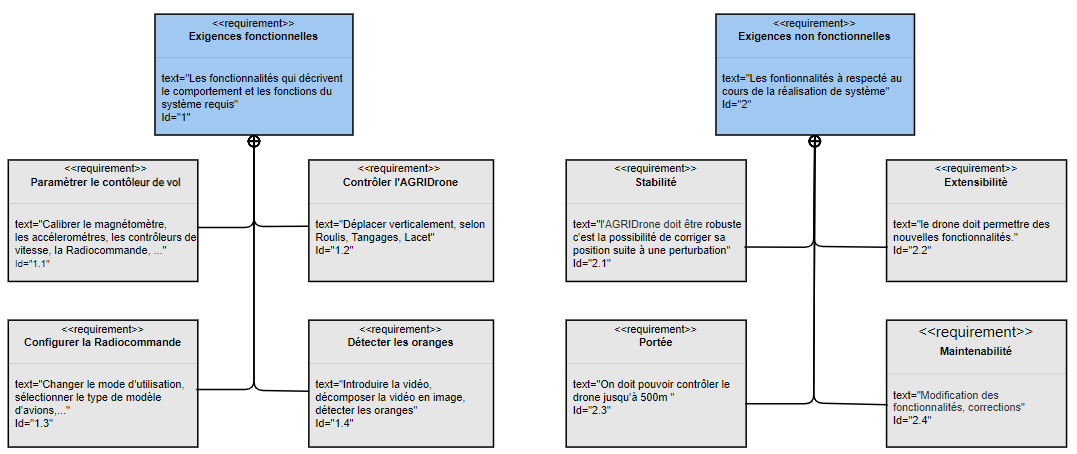
\includegraphics[width=1.2\linewidth]{Images/Diagramme d'exigence}
		\caption{Diagramme d'exigence}
	\end{center}
\end{figure}	
\section{Diagrammes des cas d'utilisation }
Cette structure est bien adaptée pour décrire de manière claire les fonctions et/ou les objectifs les plus importants d’un système[15]. Pour cette raison que l’élaboration d’un diagramme de cas d’utilisation est souvent l’une des premières étapes lors de la conception de système ou de la planification de nouveaux processus métier. 

		\subsection{Cas d'utilisation global }
		
		En se basant sur les fonctionnalités décrites ci-dessous nous précison dans ce paragraphe le diagramme de cas d'utilisation globale de notre projet. Ce diagramme est général, il traite les besoins un par un et regroupe un ensemble de fonctionnalités dans un seul cas qui peut être à son tour détaillé afin de mieux le comprendre.
		
	
		\begin{figure} [h]
		\begin{center}
			\centering	
		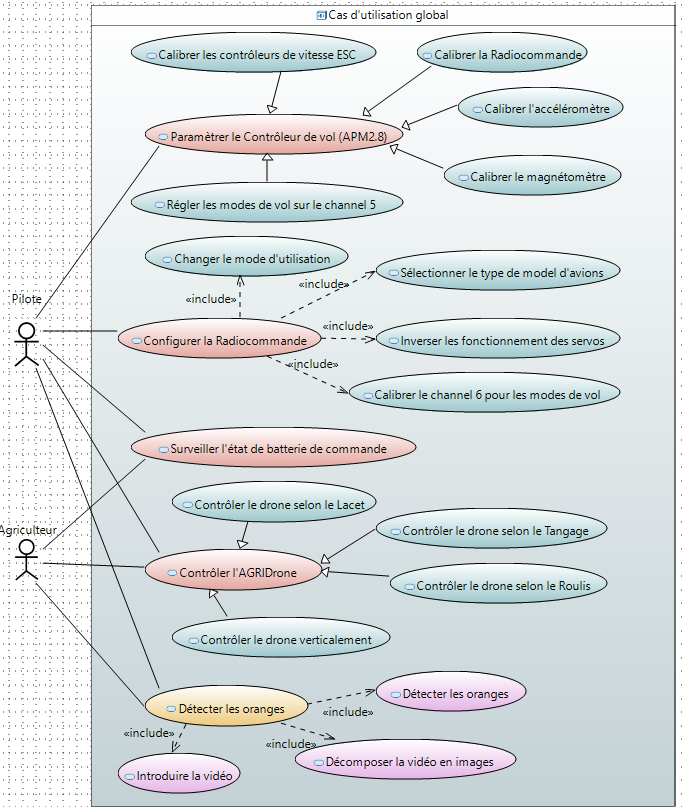
\includegraphics[width=0.9\linewidth]{Images/Diagramme de cas d'utliisation global}	
		\end{center}
		\caption{Diagramme de cas d'utilisation global}
		\end{figure}
		\newpage
		
		La figure précédente décrit d'une manière générale les différents acteurs du système ainsi que les fonctionnalités principales dont ils disposent.
		Ci-dessous, nous montrons quelques cas d'utilisation afin de mieux comprendre les fonctions attribuées à chaque acteur.
	
		\subsection{Cas d'utilisation Pilote}
		Nous montrons à travers la figure suivante le diagramme de cas d’utilisation du pilote qui permet de déterminer les principales fonctions qu’il doit effectuer. A savoir, en paramètrant le contôleur de vol, cet acteur a la possibilité de calibrer les contrôleurs de vitesses, la radiocommande, l'accéléromètre, le magnétomètre et régler les modes de vol sur le channel 5. Le pilote doit contrôler l'AGRIDrone en le déplacent verticalement, selon le lacet, le tanguage et le roulis.En plus, il surveille l'état de batterie de commande. 
		
		\begin{figure}[h] 
		\begin{center} 
			\centering
		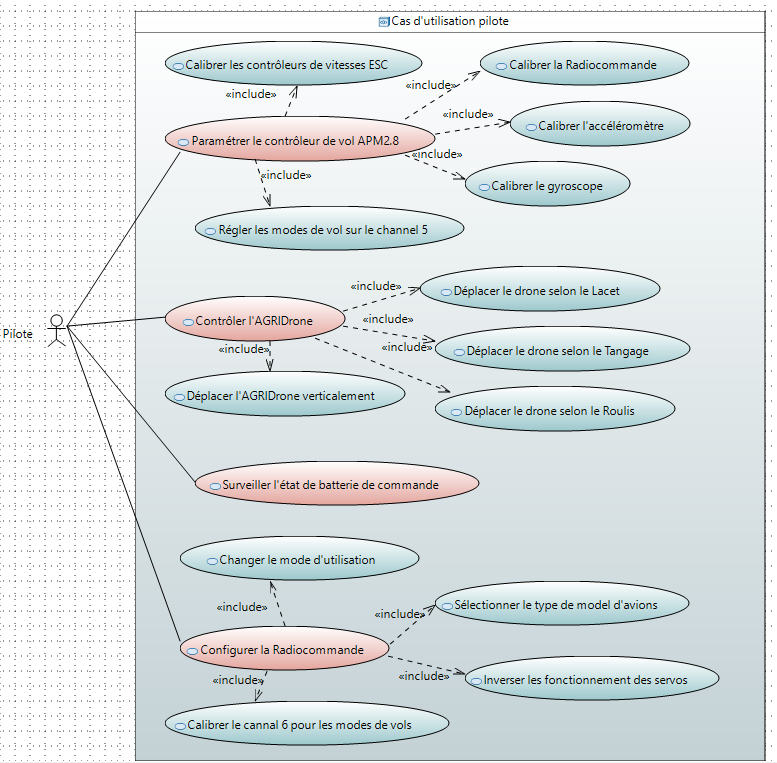
\includegraphics{Images/Diagramme de cas d'utilisation pilote}
		\end{center}
		
		\caption{Diagramme de cas d'utilasation pilote}
		\end{figure}
	
		\subsection{Cas d'utilisation d'agriculteur }
		
		\begin{figure}[h] 
		\begin{center} 
			\centering
			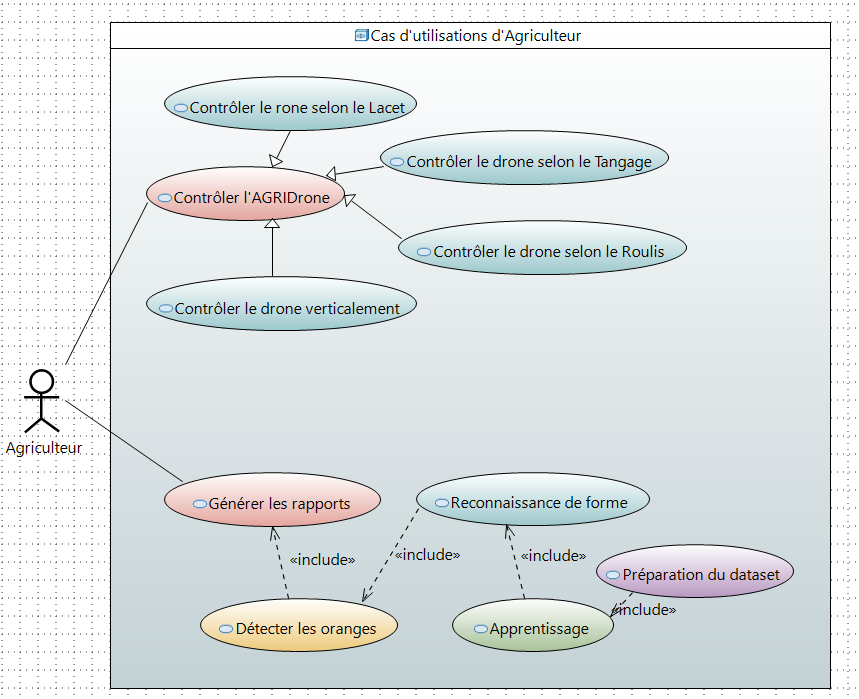
\includegraphics[width=1\linewidth]{Images/Diagramme de cas d'utilisation agriculture}
		\end{center}
		
		\caption{Diagramme de cas d'utilisation d'agriculteur}
		\end{figure}
		La figure au dessus décrit le cas d’utilisation d'agriculteur qui permet de contrôler l’AGRIDrone et surveiller le niveau d'état de batterie de commande.
	
\section{Choix d'outil de modélisation }
Avant de commencer la modélisation de notre projet, nous avons choisi un logiciel permettant de réaliser des diagrammes SysML. Après  quelques  recherches  nous avons   sélectionné:
\begin{itemize}
	\item Visual Paradigm Online ("VP Online") est un outil de création de diagrammes basé sur le Web qui prend en charge un grand nombre de diagrammes commerciaux et techniques[11]. Cet outil a été choisi pour travailler sur le diagramme d'exigence également sur le diagramme de définition de bloc.
	
	\begin{figure} [h]
		\begin{center}
			\centering	
			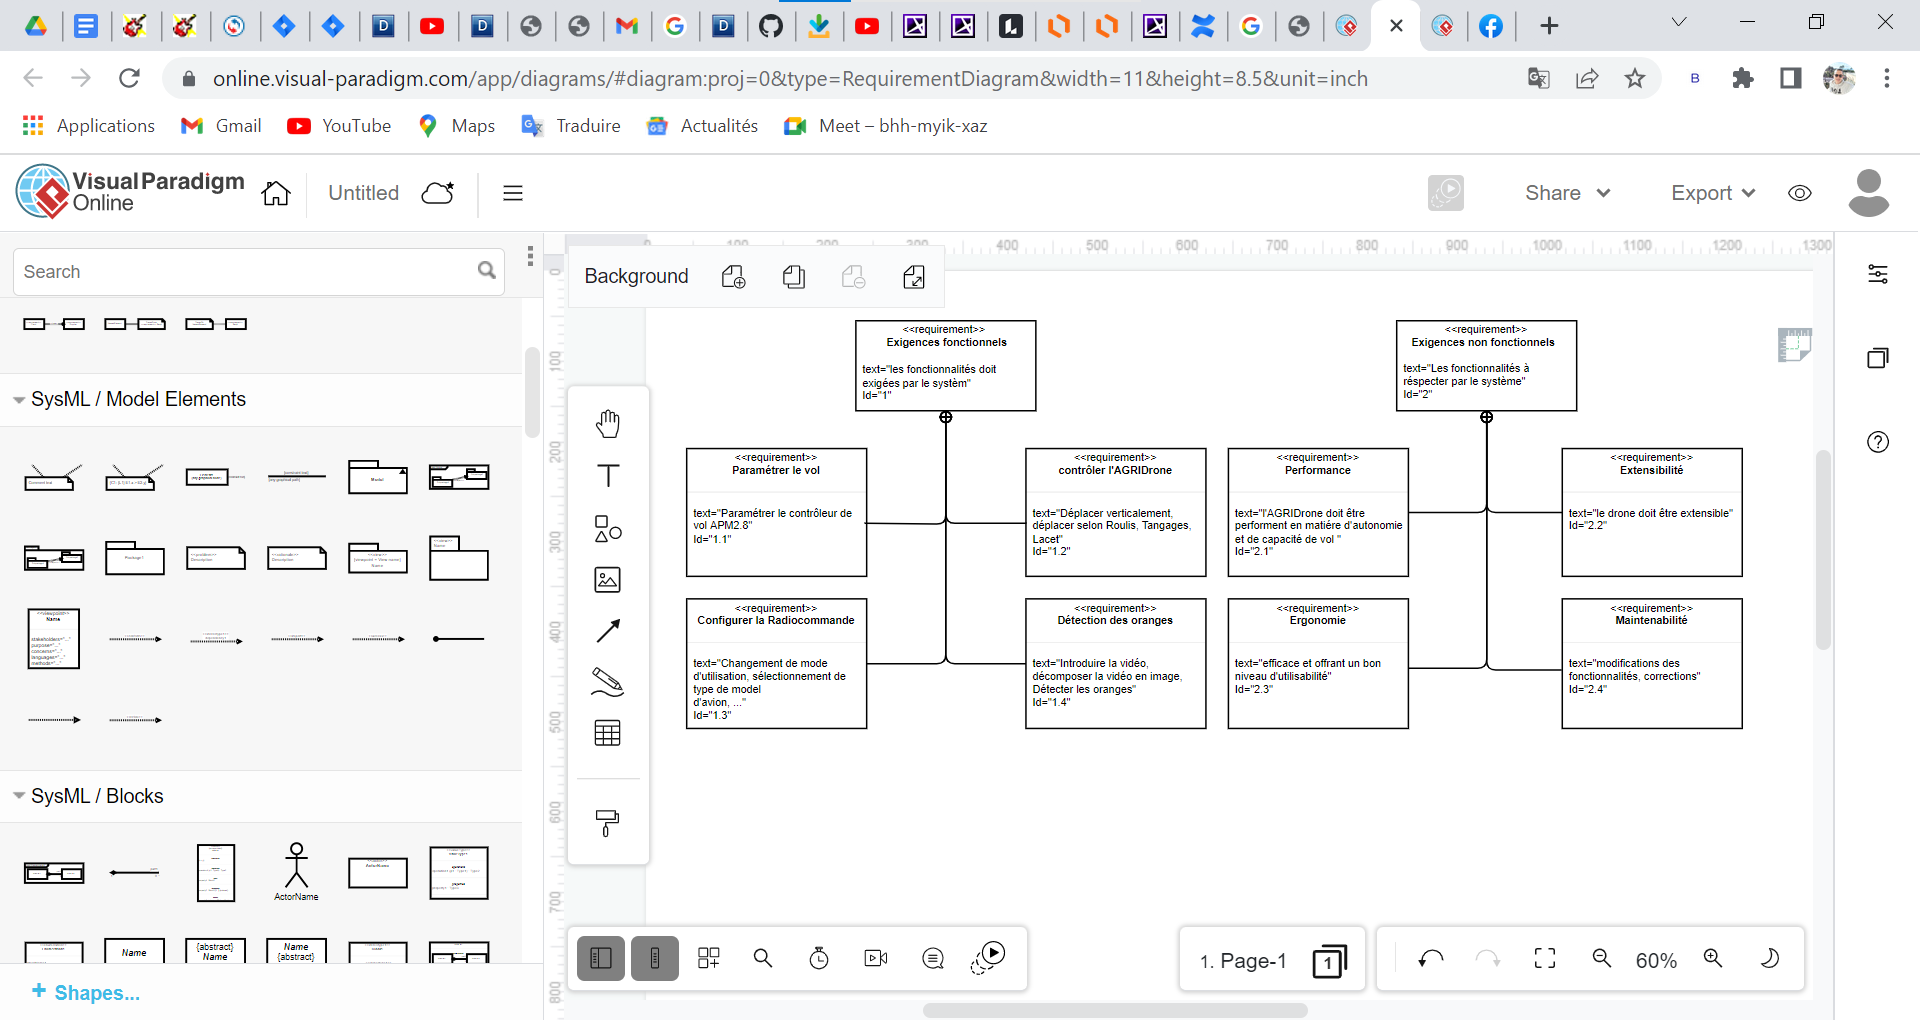
\includegraphics[width=0.8\linewidth]{Images/Visual Paradigm}
		\end{center}
		
		\caption{Vue généraliste de Visual Paradigm}
	\end{figure}
	
	
	\item Eclipse Papyrus ™ fournit un environnement intégré consommable par l'utilisateur pour l'édition de tout type de modèle EMF et en particulier pour la prise en charge d'UML et des langages de modélisation associés tels que SysML et MARTE[12]. Cet outil a été sélectionné pour travailler sur les diagrammes des cas d'utilisations.
\end{itemize}
\begin{figure} [h]
	\begin{center}
		\centering	
		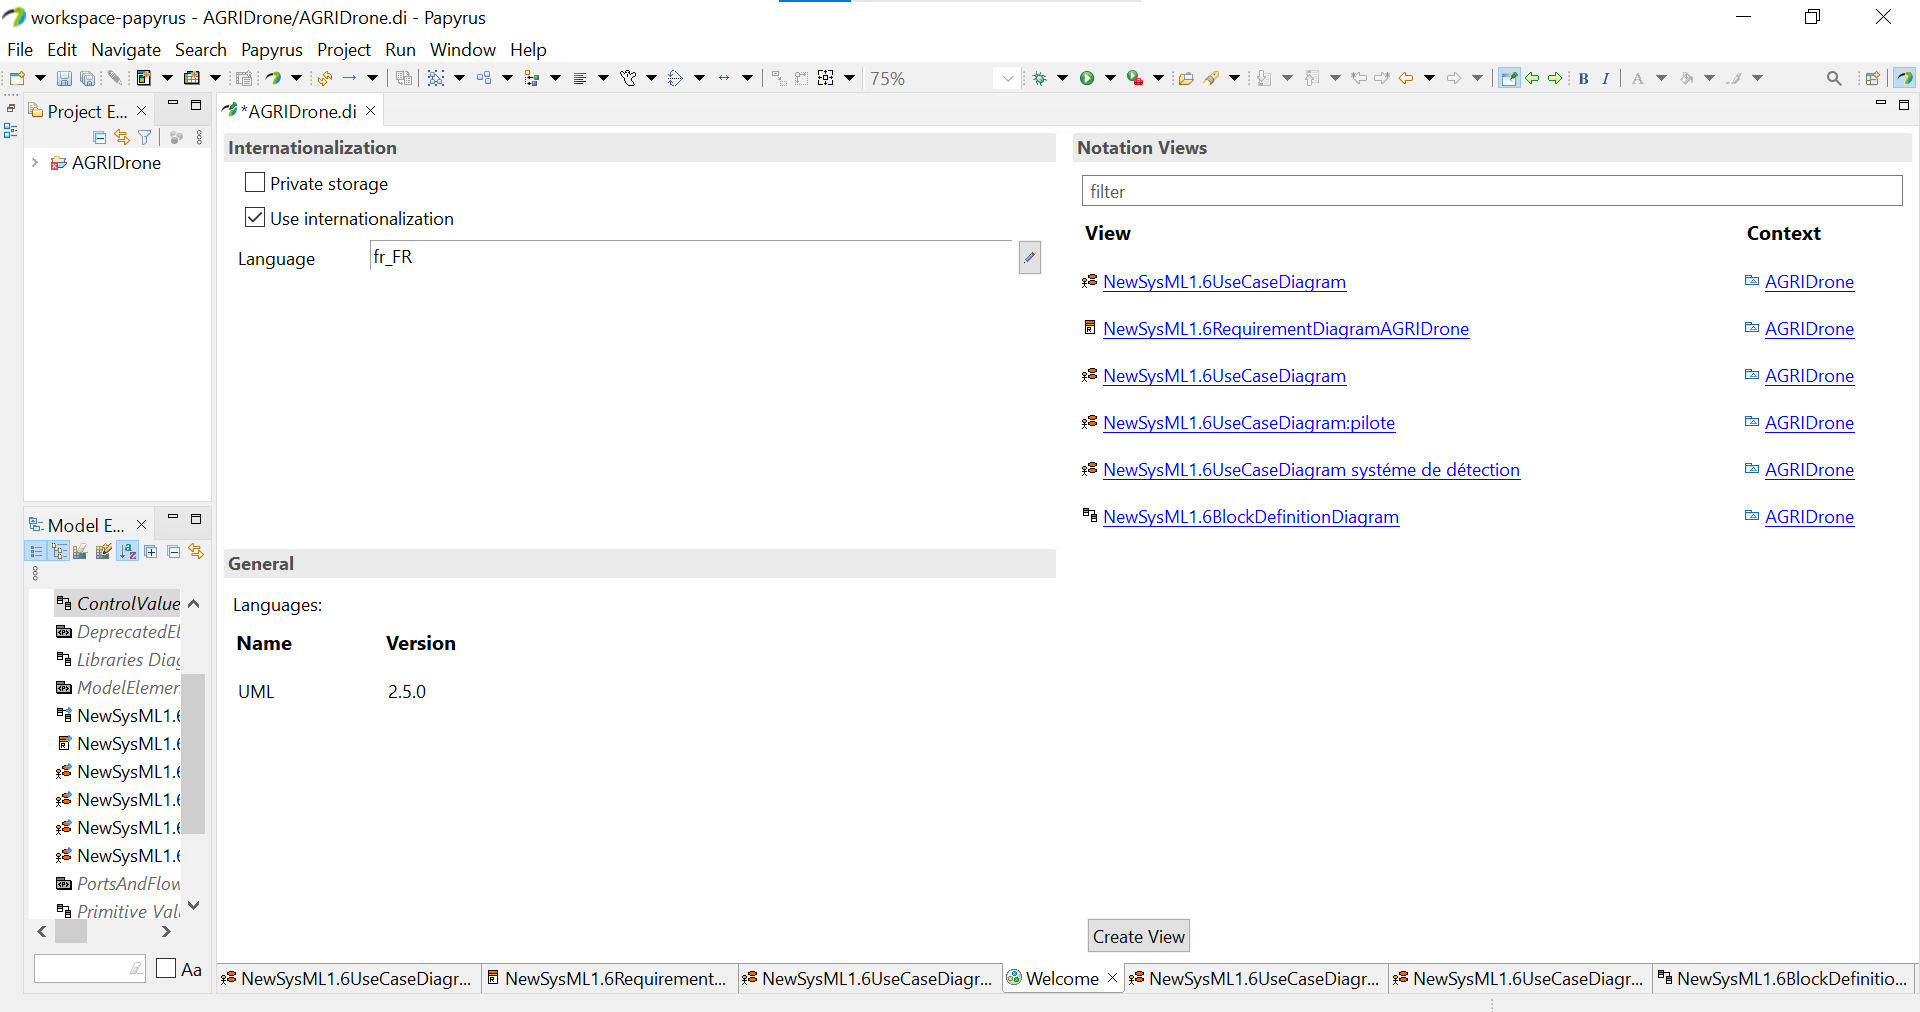
\includegraphics[width=0.8\linewidth]{Images/papyrus}
	\end{center}
	\caption{Vue généraliste de Papyrus}
\end{figure}	
\section{Conclusion}
	

	

	

